


\tikzset{
    % >=stealth'    ,
    pil/.style={ ->, thick, shorten <=0.1pt,  shorten >=0.1pt,},
    dasharrow/.style={ ->, thick, shorten <=1pt,  shorten >=1pt, dashed}, 
    %Define style for boxes
  }

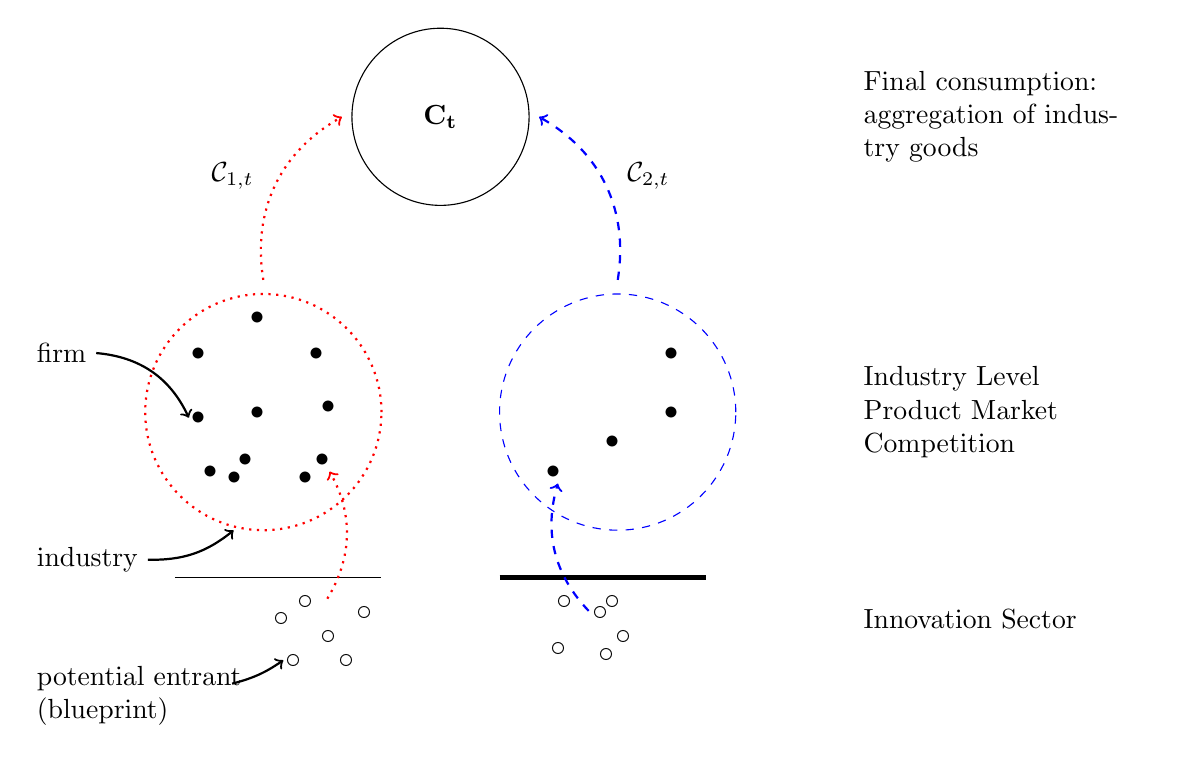
\begin{tikzpicture}[scale=0.75]


\begin{scope}[color=black]
     \draw (7,5) circle (1.5 cm);
\end{scope}

  \node (const) at (7,5)  { $\mathbf{C_t}$ };
  \node[anchor=west, text width=3.5cm] (cons) at (14,5)  { {Final consumption:\\ aggregation of industry goods}};

% differentiate industries
   \node[text width=3cm](industry1) at (4,2.4) {}; % {{\color{red} Competitive industry}};
   \node(industry2) at (10,2.4) {}; %{{\color{blue} Concentrated industry}};

% consumption from industry east
   \node (c1) at (8.5,5) {};
   \node (c2) at (10,2) {};
   \draw[pil, bend right=35, draw=blue, dashed] (industry2.south) to (c1.east);
 \node[anchor=west] (cons2) at (10,4)  { $\mathcal{C}_{2,t}$ };

% consumption from industry west
   \node (c3) at (4,2) {};
   \node (c4) at (5.5,5) {};
   \draw[pil, bend left=35, draw=red, dotted] (industry1.south) to (c4.west);
   \node[anchor=east] (cons1) at (4,4)  { $\mathcal{C}_{1,t}$ };


   \begin{scope}[color=red, dotted, thick]
        \draw (4,0) circle (2cm);
    \end{scope}

   \begin{scope}[color=blue, dashed]
        \draw (10,0cm) circle (2cm);
    \end{scope}



    % \node[anchor=south] (comp) at (2,2.5) {\centering \bfseries{Competitive {\color{red} Ind. 1}}};
    % \node[anchor=south] (conc) at (8,2.5) {\centering \bfseries{Concentrated {\color{blue} Ind. 2}}};
    \node[anchor=west, text width=3cm] (cons) at (14,0)  { {Industry Level Product Market Competition}};



%firms in first industry circle
% \uncover<3-> {
    \node (11) at (5,1)  {\circle*{4}};
    \node (12) at (3,-0.1) {\circle*{4}};
    \node (13) at (5.1,-0.8) {\circle*{4}};
    \node (14) at (3.6,-1.1) {\circle*{4}};
    \node (15) at (4,1.6) {\circle*{4}};
    \node (16) at (4,0) {\circle*{4}};
    \node (17) at (3.8,-0.8) {\circle*{4}};
    \node (18) at (3.2,-1) {\circle*{4}};
    \node (19) at (4.8,-1.1) {\circle*{4}};
    \node (110) at (3,1) {\circle*{4}};
    \node (111) at (5.2,0.1) {\circle*{4}};
  
%firms in second industry circle
    \node (21) at (11,1) {\circle*{4}};
    \node (22) at (9,-1) {\circle*{4}};
  %  \node (23) at (7.6,1.6) {\circle*{4}};
    \node (24) at (10,-.5) {\circle*{4}};
    \node (25) at (11,0) {\circle*{4}};

    % \node (dummy11) at (8,1) {};
   \node[anchor=west] (omega11) at (0,1) {firm} ;
   \draw[pil, bend left=30 ] (omega11.east) to (12.west);

   \node[anchor=west] (omega12) at (0,-2.5) {industry} ;
   \draw[pil, bend right=20 ] (omega12.east) to (3.5,-2cm);


%innovators
   \draw[thin]  (2.5,-2.8)--(6,-2.8); 
   \draw[ultra thick] (8,-2.8)--(11.5,-2.8);

    \node (31) at (4.8,-3.2) {\circle{4}}; 
    \node (32) at (4.4,-3.5) {\circle{4}};
    \node (33) at (5.2,-3.8) {\circle{4}};
    \node (34) at (5.8,-3.4) {\circle{4}};
    \node (35) at (4.6,-4.2) {\circle{4}};
    \node (36) at (5.5,-4.2) {\circle{4}};

    
    \node (37) at (10,-3.2) {\circle{4}}; 
    \node (39) at (10.2,-3.8) {\circle{4}};
    \node (310) at (9.8,-3.4) {\circle{4}};
    \node (312) at (9.9,-4.1) {\circle{4}};
    \node (313) at (9.1,-4) {\circle{4}};
    \node (314) at (9.2,-3.2) {\circle{4}};

   \node[anchor=west, text width=3cm,] (omega13)  at (0,-4.8) {potential entrant \\(blueprint)} ;
   \node                               (omega13b) at (3.3,-4.6) {} ;
   \draw[pil, bend right=10 ] (omega13b.east) to (35.west);


    \draw[dasharrow, bend right=30, draw=red, dotted] (31.east) to (13.south);
    \draw[dasharrow, bend left=30, draw=blue, dashed] (310.west) to (22.south);

    \node [anchor=west, text width=3.5cm, ] (innov) at (14,-3.5) {Innovation Sector}; 



\end{tikzpicture}
